% This must be in the first 5 lines to tell arXiv to use pdfLaTeX, which is strongly recommended.
\pdfoutput=1
% In particular, the hyperref package requires pdfLaTeX in order to break URLs across lines.

\documentclass[11pt]{article}

% Remove the "review" option to generate the final version.
\usepackage[review]{ACL2023}

% Standard package includes
\usepackage{times}
\usepackage{latexsym}

% For proper rendering and hyphenation of words containing Latin characters (including in bib files)
\usepackage[T1]{fontenc}
% For Vietnamese characters
% \usepackage[T5]{fontenc}
% See https://www.latex-project.org/help/documentation/encguide.pdf for other character sets

% This assumes your files are encoded as UTF8
\usepackage[utf8]{inputenc}

% This is not strictly necessary, and may be commented out.
% However, it will improve the layout of the manuscript,
% and will typically save some space.
\usepackage{microtype}

% This is also not strictly necessary, and may be commented out.
% However, it will improve the aesthetics of text in
% the typewriter font.
\usepackage{inconsolata}

%% Use the graphicx package to include figures.
\usepackage{graphicx}
\usepackage{caption}
\usepackage{subcaption}
\usepackage{placeins}
\usepackage{fancyvrb}
\usepackage{amsmath}

\DeclareMathOperator*{\argmax}{arg\,max}
\DeclareMathOperator*{\argmin}{arg\,min}
% If the title and author information does not fit in the area allocated, uncomment the following
%
%\setlength\titlebox{<dim>}
%
% and set <dim> to something 5cm or larger.

\title{Examining Calibration Large Language Model in Question Answering}

% Author information can be set in various styles:
% For several authors from the same institution:
% \author{Author 1 \and ... \and Author n \\
%         Address line \\ ... \\ Address line}
% if the names do not fit well on one line use
%         Author 1 \\ {\bf Author 2} \\ ... \\ {\bf Author n} \\
% For authors from different institutions:
% \author{Author 1 \\ Address line \\  ... \\ Address line
%         \And  ... \And
%         Author n \\ Address line \\ ... \\ Address line}
% To start a seperate ``row'' of authors use \AND, as in
% \author{Author 1 \\ Address line \\  ... \\ Address line
%         \AND
%         Author 2 \\ Address line \\ ... \\ Address line \And
%         Author 3 \\ Address line \\ ... \\ Address line}

%\author{Aakarsh Nair\\
%  University of Tuebingen / Geschwister-Scholl-Platz, 72074 Tübingen\\
%  \texttt{aakarsh.nair@student.uni-tuebingen.de} \\
%  Béla Linus Rösener \\
%  University of Tuebingen / Geschwister-Scholl-Platz, 72074 Tübingen\\
%  \texttt{linus.roesener@student.uni-tuebingen.de} \\
%  Yin-Yin Cheng \\
%  University of Tuebingen / Geschwister-Scholl-Platz, 72074 Tübingen\\
%  \texttt{yin-yin.cheng@student.uni-tuebingen.de}
%  }
\author{Aakarsh Nair 
    \and Béla Linus Rösener 
    \and Ilinca Vandici  
    \and Yin-Yin Cheng 
    \and Adne Jossing \\
        Reinforcement Learning for Large Language Models\\
        Seminar für Sprachwissenschaft,  Eberhard Karls Universität Tübingen \\
 Keplerstraße 2, 72074 Tübingen, Germany\\
        \{firstName.lastName\}@student.uni-tuebingen.de
}


\begin{document}
{\makeatletter\acl@finalcopytrue
  \maketitle
}
%\maketitle

%% Abstract: Short summary of the paper (up to 150 words), 
%% should include the conclusion of your study.

\begin{abstract}
In this paper, we examine the issue of calibration of 
large language models. 
That is the relationship between the \emph{confidence} 
of a predicted answer on a question-answering task 
with its \emph{empirical likelihood of being correct}.

We replicate elements of previous calibration study 
\cite{kadavath2022language} on several multiple-choice 
(MMLU, LogicQA, TruthfulQA) 

We find that models do scale in their calibration ability by 
model size. Moreover models fine-tuned as conversation agents 
do improve in their calibration and accuracy under 
few-shot prompting. 

However, we also observe that for tasks beyond models reasoning 
capability (complex logical and scientific reasoning) fine-tuning 
harms model's accuracy and leads to overconfidence 
in model predictions.

\end{abstract}


\section{Introduction}

%% Introduction: Introduction, Motivation and explanation of
%% the research question in the \emph{context of the field}/the 
%% class, explaining why it is interesting/novel in 
%% comparison to extant related work. Note that it is NOT 
%% mandatory to include an exhaustive literature review; 
%% it is sufficient to mention relevant work from the project 
%% proposals and the class materials.

Understanding the reliability and correctness of language model (LM) 
generations is crucial in ensuring their practical utility and trustworthiness.  Trustworthiness requires that the language model 
produce not just grammatically correct sentences, but sentences 
which accurately reflect the language models' understanding 
of the state of the world as well as the its understanding as to 
the limits its ability reason based on its current 
internal knowledge about the question at hand. Calibration is a metric commonly used to quantify such a relationship. 

Where calibration refers to the relationship between 
the language model's \emph{confidence} of a predicted answer 
on a question-answering task being correct with 
its  \emph{empirical likelihood} of actually being  
correct. In the case of a perfectly calibrated model, the relationship is linear \cite{spiess2024quality}. 

Several observations have been made on the topic of calibration in LLMs specifically. Kadavath et al. finds that the probabilities assigned to answer options on benchmark datasets seem to correlate with correctness probabilities, a tendency which is especially visible for the results obtained by bigger models \cite{kadavath2022language}. They also mention that while LLMs are generally well-calibrated, the use of reinforcement learning can sometimes damage calibration, but that a temperature adjustment seems to do the trick in replacing the model on the path of correct calibration.

In this study, we aim to replicate the findings of Kadavath et al., focusing on obtaining calibration measures for different LLama models \cite{touvron2023llama} of different sizes, datasets pertaining to a variety of tasks (general question answering, logic), in order to gain a more complete understanding of the factors that might influence an LLM's calibration, as well as the challenges they present.



\section{Methods}

%% Methods: Detailed description of the study addressing the 
%% research question (including all details of, e.g., 
%% the models, datasets, used analyses, etc...). 
%% It should enable another person reading your paper to *fully*
%% replicate the study. *No results* or *interpretation* 
%% should be included yet.

\subsection{Introduction}
%% TODO: Not enough mathematical explanation of what the term mean. 
%% TODO: Not explaining, what log completion probbilty means. 
%% TODO: No explantation of transfoerm completion. 

We measure the calibration in keeping with the methodology 
presented in \cite{kadavath2022language}. 

\subsection{Inference Datasets}

In order to understand the the behavior of base vs fine-tuned chat models 
(models fine tuned as conversational agents). We test out models of varying sizes 
(7b, 13b and in some cases 70b parameters) on a variety of question answering datasets. 
A brief explanation of the datasets used is given here:

\subsubsection{MMLU}

The Measuring Massive Multitask Language Understanding (MMLU) 
\cite{hendryckstest2021} \cite{hendrycks2021ethics} is a massive dataset of 
multiple choice questions which covers 57 tasks in various subjects including elementary mathematics, 
US history, computer science, law, and more. For convenience the datasets are grouped into 
four categories \emph{STEM}, \emph{Humanities}, \emph{Social Sciences}, 
and \emph{Other}(global facts, marketing, accounting etc.). 
Questions test the model for both factual and conceptual understanding 
of the given topics.

\subsubsection{LogicQA}

LogicQA \cite{liu2020logiqa} is a comprehensive dataset, which is sourced 
from expert-written questions for testing human logical reasoning. It consists of 8,678 QA 
instances, covering multiple types of deductive reasoning. Neural modes 
still lag human performance on these questions.

\subsubsection{TruthfulQA}

TruthfulQA \cite{lin2021truthfulqa} is a benchmark to measure whether 
a language model is truthful in generating answers to questions. The benchmark comprises 
817 questions that span 38 categories, including health, law, finance and politics. 
Questions are crafted so that some humans would answer falsely due to a false belief or misconception. 
To perform well, models must avoid generating false answers learned from imitating human texts. These 
datasets are especially hard for language models 
to be accurate can reveal case where accuracy 
and calibration for a model might deviate. 


\subsection{Multiple Choice Query Format}

As language models can be sensitive to prompting formats we breifly describe our question-answering format for multiple choice questions.

MMLU, LogicQA and TruthfulQA datasets provide a set of 
options for each question in their dataset along with 
the most appropriate answer. The choices provided 
are converted are multiple choice question format 
with lettered set of options next to each possible answer followed by the answer prompt. 
A sample question prompt is shown in Figure \ref{fig:mmlu-sample-question}.

\begin{figure}
\begin{Verbatim}
This question refers to the following 
information.

To him I shall come when I go beyond this 
life, and to him will come he who has faith 
and doubts not.
—The Upanishads, India, c. 1000 BCE

To which religion does the speaker most 
likely belong?

(A). Hinduism
(B). Buddhism
(C). Shintoism
(D). Zoroastrianism

Answer:
\end{Verbatim}
\caption{Sample Question from MMLU Dataset}
\label{fig:mmlu-sample-question}
\end{figure}

Constraining the model generation to one of these options 
allows us to judge the relative probability of each the answer completions by 
looking at the token completion probability 
for each of the  formatted options $(A),(B) \dots (D)$ 
respectively. 
In a few shot example we include multiple questions 
with the answer completion filled in after the prompt which allows the model to understand the answer 
format.

The model is queried in either a \emph{0-shot} or 
\emph{few-shot} manner. In the few-shot questioning, in 
addition to the question under test we precede the question 
with additional questions in the same multiple choice format 
in order to provide the model with enough context 
to understand the expected format for answering the questions.

\iffalse
\subsubsection{Completion Questions} %% TODO: Fix

For completion oriented datasets such as HumanEval and GSM8k which 
contain a prompt and a 'canonical answer' for each prompt. In order to 
translate this into a prompt format based on which we can obtain easily 
interpretable results, we follow the approach of Kadavath, prompting 
the model with both the prompt and the canonical answer, asking the 
model to choose between True and False. However, since this only 
evaluates whether the model can generate an output based on correct 
prompts, we also shuffle the dataset in order to also provide the model 
with instances where the canonical answer does not match the prompt 
and is therefore incorrect. 

Moreover, we also explore the model's performance with another prompt format (which we only tested on the Humaneval dataset, due to technical limitations). For this part of the experiment, we provide the model with the prompt and lettered options (all extracted from the dataset, one of which is the correct answer and the other ones being retrieved at other indexes), replicating pattern similar to the MMLU dataset. We also run the experiment adding a 'None of the above' option to see if it destabilizes calibration in the same way it does for the MMLU dataset.
\fi


\subsection{Models}

The tests are conducted on variants of the  open source LLama 
Language Models from Meta \cite{touvron2023llama}. The LLama Language model 
uses a transformer based architecture described in first described in 
\cite{VaswaniSPUJGKP17} trained on the next-token prediction task on 
textual datasets. All the model weights as well as the datasets it has 
been trained on are publicly available. These include large texts from  
datasets like CommonCrawl, Wikipedia, Github and Gutenberg and other 
open datasets. 

The model comes in two variants \emph{base} and \emph{chat} of three 
model sizes $7b$, $13b$ and $70b$ referring to the number of weights/parameters in billions, 
in each model class. These allow users to trade off model accuracy for inference speed 
and computational resources required run each of the models. 

The \emph{chat} model is a fine tuned version of the 
corresponding \emph{base} model. It has been fine tuned using 
RLHF as described in \cite{ouyang2022training} to act 
as a helpful conversational agent.

Most of the experiments in this paper are conducted on the model 
with $7b$ weights on the \emph{base} and \emph{chat} versions of 
the model. Additional model weights ($13b$ or $70b$) 
are used when possible to demonstrate effects of scaling the model on accuracy and calibration.

\subsubsection{Computing Probability of Completion}

For each question and a particular possible completion 
(for example $(A), (B), \dots (D)$)  we tokenize the concatenated 
prompt completion/answer pair and run inference on the full completion. 
The model output's logits give us the scores of the each 
possible token at every position. 

We convert the logits into log-probabilities and extract the probabilities for 
isolated segment containing just the completion and compute the mean of this segment to 
normalize for completions of different length (For most of our multiple choice cases 
the expected completion is simply the alphanumeric option $(A), (B), \dots $ 
thus our completions are of the same length).

Having obtained the log-probability for each completions we convert these to 
a normalized probability by applying a \emph{softmax} over the log-probabilities 
for each completion. 

The model selected option is considered to be the maximum over 
these probable answers. 

\begin{equation}
    o_{selected} = \argmax_{o_i \in l_A, l_B, \dots}  
    \frac{e^{o_i}}{\sum_{o_j \in l_A, l_B, l_C, \dots} e^{o_j}} 
\end{equation}

Where $l_A, l_B\dots$ are the corresponding log probabilities of the selected completions/answers.

\subsection{Computing Calibration and Accuracy}

Given the selected answer along with the probabilities 
of the answers which have not been selected we can 
compute the calibration of the model.  That is the relationship 
between the \emph{confidence} of a predicted answer on a 
question-answering task with its \emph{empirical likelihood of being correct}, 
using the selected answer and probabilities for all answers which were not-selected. 
Following the \cite{kadavath2022language}, selected answers and their 
probabilities are sorted and distributed into bins containing equal number of samples.

\subsubsection{Calibration Plots}

We can compute and compare the  empirical estimate of the 
probability of the answer in a bin being correct, with the model 
predicted probability of the answer. For ideal calibration, that 
is when the model completion probability aligns closely with the 
empirically estimated probability of answering the question correctly, 
these  two computed probabilities must be equal. 
Thus an ideal calibration would be represented by a line of 
slope $1$ in on a calibration plot.

We plot these two probabilities we find that for bins 
where the model \emph{over-confident} its expected 
probabilities will be larger than the empirical probabilities 
thus reflected in the ratio lying below the ideal calibration 
line and when the model is \emph{under-confident} its 
expected probabilities will be less than its empirical  
probabilities with the ratio above the 
ideal calibration line.

\subsubsection{Accuracy Characterization}

We characterize model's ability to discriminate between questions it 
knows the answer to against ones it doesn't  by using the area under 
its receiver operating characteristic curve (\textbf{AUROC}). 
A discriminator with \textbf{AUROC}  close to 0.5 would have 
chance accuracy with 1 being the best. As \textbf{AUROC} is 
indifferent to calibration. We can test the model's accuracy 
and calibration independently across different datasets of 
different sizes.

\subsubsection{Calibration Error}

Metrics \textbf{Expected calibration error(ECE)} and \textbf{RMS calibration error (RMSE)} are computed as in \cite{kadavath2022language}. 

\begin{equation}
    E_{ECE} = \frac{1}{N}  \sum_{i}^N | p_{model} - p_{empirical}|
\end{equation}

\begin{equation}
    E_{RSME} = \sum_{i}^N \sqrt{\frac{1}{N} (p_{model} - p_{empirical})^2}
\end{equation}

Where $N$ stands for the number of bins and is set to the standard $10$ bins. We only consider 
the probability of the model's predicted answer in computing these metrics. 
Visual calibration plots however are overall found to be more 
informative as to models' calibration behavior than these summary statistics.

\section{Results}

%% Results: Results of the study, presented, e.g., 
%% as a table, figure or described in words, description of 
%% the results of statistical analyses (if applicable). 
%% An interpretation with respect to the research 
%% question and the tested hypotheses should be 
%% included.

%% \subsection{Introduction}


\subsection{Model Calibration Results on MMLU}

Running the above calibration experiment on the entire 
MMLU dataset on the models of size $7b$, $13b$, and $70b$ 
we can make some key observation. 

\subsubsection{Zero Shot Settings}

We begin by noting that base models $7b, 13b$ tend to be 
\emph{under-confident} in their predicted probabilities, while 
the chat models  for $7b, 13b$ tend to be  \emph{overconfident}.
However the overall calibration error of both base and chat
models is fairly close. See Figure \ref{fig:0-shot-MMLU}  for 
the corresponding calibration plot. We note that $70 b$ model is well 
calibrated out of the box without any fine-tuning. This leads us to 
hypothesize that larger models may require less fine tuning than smaller 
models due to better prompt and contextual understanding.

In terms of accuracy we find that that, \emph{AUROC} 
of fine-tuned models is comparable or slightly lower 
or comparable to the accuracy of base models. See 
Figure \ref{fig:0-shot-MMLU-roc}.

\begin{figure*}
     \centering
     \begin{subfigure}[b]{0.60\textwidth}
         \centering 
         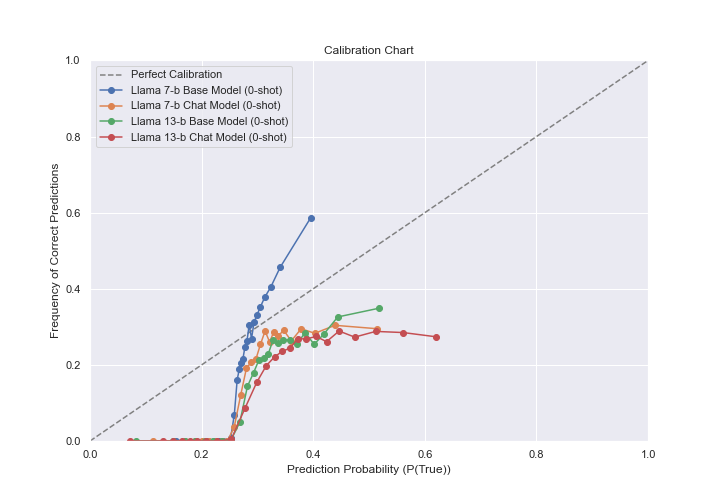
\includegraphics[width=1.1\textwidth]{figures/0-shot-MMLU.png}
         \caption{\textbf{0-shot MMLU} }
         \label{fig:0-shot-MMLU}
     \end{subfigure}
     \hfill
         \begin{subfigure}[b]{0.38\textwidth}
         \centering 
         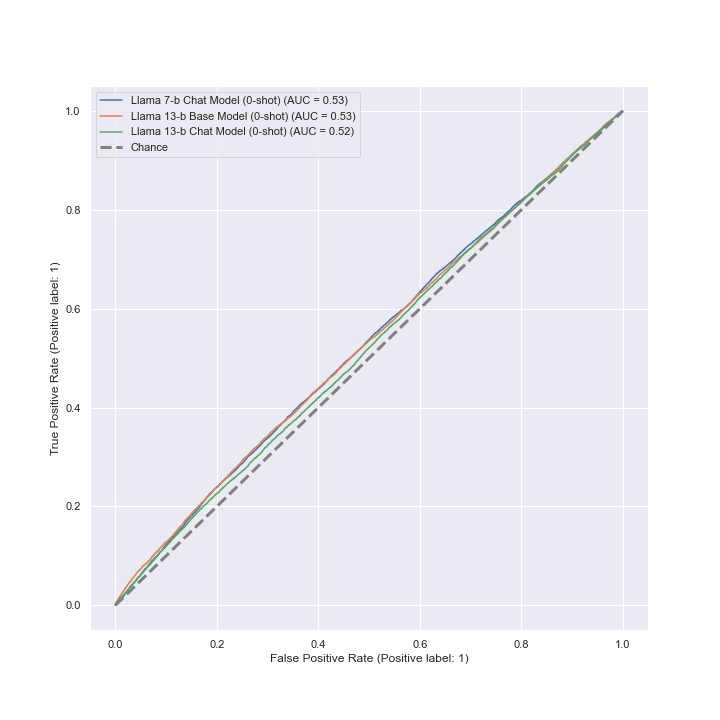
\includegraphics[width=0.9\textwidth]{figures/0-shot-MMLU-roc.png}
         \caption{\textbf{0-shot MMLU ROC}}
         \label{fig:0-shot-MMLU-roc}
    \end{subfigure}  
     \hfill
     \begin{subfigure}[b]{0.60\textwidth}
         \centering
         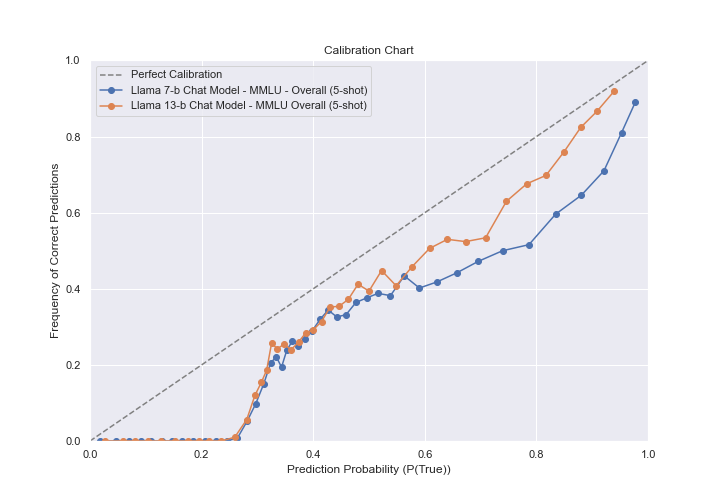
\includegraphics[width=1.1\textwidth]{figures/5-shot-MMLU.png}
         \caption{\textbf{5-shot-MMLU} }
         \label{fig:5-shot-MMLU}
     \end{subfigure}     
     \begin{subfigure}[b]{0.38\textwidth}
         \centering 
         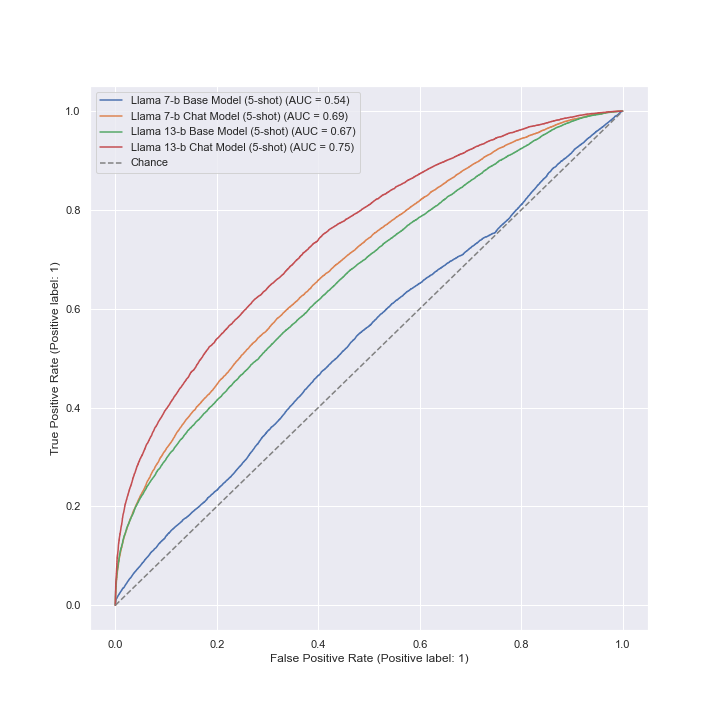
\includegraphics[width=0.9\textwidth]{figures/5-shot-MMLU-roc.png}
         \caption{\textbf{5-shot MMLU ROC} }
         \label{fig:5-shot-MMLU-roc}
    \end{subfigure} 
    
        \caption{\textbf{Calibration and Accuracy on MMLU Dataset:}. We note that few-shot prompting leads to greater accuracy and calibration for fine-tuned chat models. Without fine-tuning base models under-predict their selecting the correct answer. The AUROC curves for base models is greater than those for corresponding fine-tuned models under 0-shot prompting. However in few-shot prompting fine-tuned models perform better than base models in both calibration and accuracy. Additionally a sufficiently large chat model for example 70b chat model is able to display good calibration regardless of few-shot prompting.}
        
        \label{fig:0-5-shot-MMLU}
\end{figure*}
\FloatBarrier


\subsection{Few-shot Settings}

Our most striking and consistent observation across datasets is that model prompting has a drastic effect on fine-tuned chat model's calibration and accuracy, such that a fine-tuned $7 b$ model has a lower calibration error than even a $13 b$ base model 
under  few-shot prompting. See Figure \ref{fig:5-shot-MMLU}.


\subsubsection{MMLU Subject-Wise Calibration}

Drilling in further into a subject-wise breakdown of 
MMLU performance  Figure \ref{fig:MMLU-subjects-7b} and 
Figure \ref{fig:0-5-shot-MMLU-subjects-13b}. We begin by noting that increases 
in model size do not lead to uniform improvement across specific 
fields of MMLU. 

We note that accuracy improvements between $7b$ and 
$13b$ are roughly monotonic. Fields like 
\emph{Social Studies}, and \emph{Other} where the 
model shows high accuracy are also the fields which benefit from increased model size.

Additionally, we note that that these high accuracy fields are  also the ones which showed the lowest calibration errors under few-shot testing.

\subsection{Logic QA}

Unlike the MMLU dataset which relies heavily on factual 
knowledge, LogicQA dataset is constructed to rely 
on requiring the model to perform multiple 
logical reasoning and inference steps. 

Consequently we find that accuracy and 
calibration on  these data sets is markedly lower 
than on MMLU.  Moreover we find accuracy of 
$7b$ and $13b$ models scales shows slower 
improvement with increases  in model size. 
See Figure \ref{fig:logic-qa}.

We do still find the major trends observed in 
MMLU also hold for LogicQA. That is few-shot 
prompting leads better calibration. 

The gain in accuracy of the $13b$ fine-tuned 
chat model is minimal going from and AUROC of 
$0.68$ to $0.69$. Thus most of the gains of 
fine-tuning  this model in its improved 
calibration error between $0$-shot and 
few-shot prompting. For example the $13b$ 
chat model sees a calibration in RMSE 
of $0.39$ to $0.25$ with few-shot 
prompting. 

Furthermore while the accuracy improvements 
between $13b$ (AUROC $.69$) and $7b$(AUROC $.65$) 
chat models are not significant the $70b$ chat 
model still able to improve on this accuracy 
(AUROC of $.78$). This makes us  hypothesize that while scaling is harder on the LogicQA sufficiently large models can still learn to perform well on this dataset.

\subsection{Truthful QA}

Of the datasets under test Truthful QA turns out to be 
the hardest dataset to improve on either accuracy 
or calibration. The dataset tests models  on 
their ability to avoid reproducing human 
misconceptions and conspiracies. 

Firstly, we note that that the model scaling fails 
to produce sufficient improvements in accuracy a $13b$  
fine-tuned chat model has a AUROC of just $0.56$ where 
$.5$ chance accuracy.  

Moreover while the accuracy of the model under 
fine-tuning improves only marginally and the overall 
ECE and  RMSE calibration scores of these fine-tuned models are only marginally better than their base variants, the fine tuned model is much 
more likely be overconfident on a subset of question than their base variants.  See Figure \ref{fig:5-shot-TruthfulQA}. As our benchmark figures for 
TruthfulQA lower than reported results it remains unclear if model size is a limiting factor on this dataset.


\section{Discussion}
%%  Discussion: reflection on the results in light of the 
%% research question, discussion of limitations of the current 
%% study and possible future directions for research. 
%% What worked, what didn’t (why, if you have ideas)? 
%% This could include ideas that you had during the 
%% project that you think would be interesting to explore.


%% Conclusion (optional, could be combined with the discussion)

In this study we attempted to study language model calibration  under various 
conditions such as model size, fine tuning and task specialization. We find that 
we were able to replicate the observed  calibration behavior of closed source models like 
GPT-3, and  Claude on the open models like Llama base and fine-tuned chat variants. 

On LogicQA, MMLU datasets we find that fine-tuned chat models are better calibrated than their base variants.
We find that these fine-tuned chat models respond very well to few-shot prompting, with their accuracy and calibration improving significantly from 0-shot to 5-shot prompting. Additionally simply increasing 
model size going from 7b to 13b to 70b increases model's accuracy and calibration. Inside of MMLU dataset we find  STEM dataset remains hardest in terms both accuracy and calibration though we do see improvements with larger model sizes.

On difficult datasets such as TruthfulQA, where the 
model is not able to attain high accuracy, fine-tuning 
increase model's confidence without the corresponding 
increase in accuracy. This leads us to believe that 
calibration is fundamentally limited by model 
expressiveness for some subset of questions. Here 
the model cannot, \emph{know that it doesn't know}. It remains unclear if this is a limitation of model size or a fundamental limitation of the model itself.  


\begin{figure*}
     \centering
     \begin{subfigure}[b]{0.60\textwidth}
         \centering 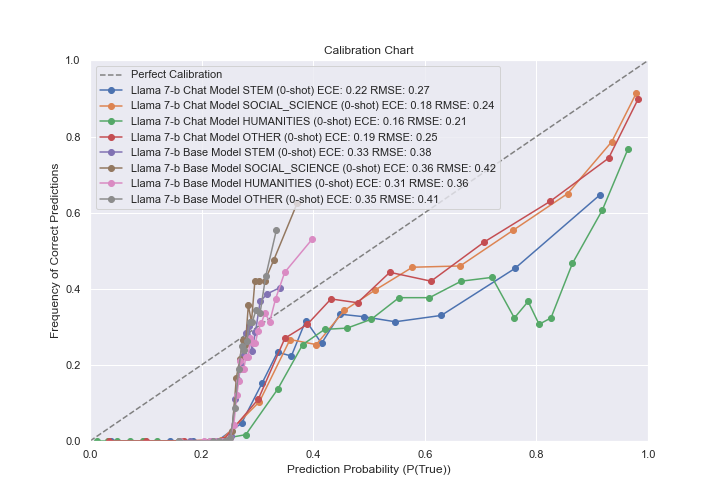
\includegraphics[width=1.1\textwidth]{figures/0-shot-MMLU-subjects-7b.png}
         \caption{\textbf{0-shot MMLU by Subject(7b):} }
         \label{fig:0-shot-MMLU-subjects-7b}
     \end{subfigure}
     \hfill
     \begin{subfigure}[b]{0.38\textwidth}
         \centering 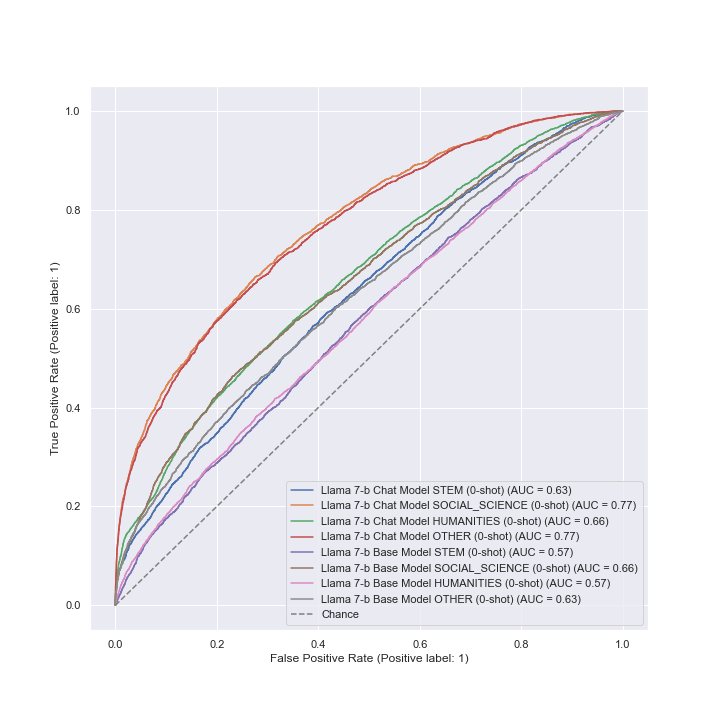
\includegraphics[width=0.9\textwidth]{figures/0-shot-MMLU-subjects-7b-roc.png}
         \caption{\textbf{0-shot MMLU by Subject ROC (7b):} Performance on MMLU shows poor classification, however few-shot prompting enhances classification for subjects the model is predisposed to answer}
         \label{fig:0-shot-MMLU-subjects-7b-roc}
    \end{subfigure}
    
     \hfill
     \begin{subfigure}[b]{0.60\textwidth}
         \centering
         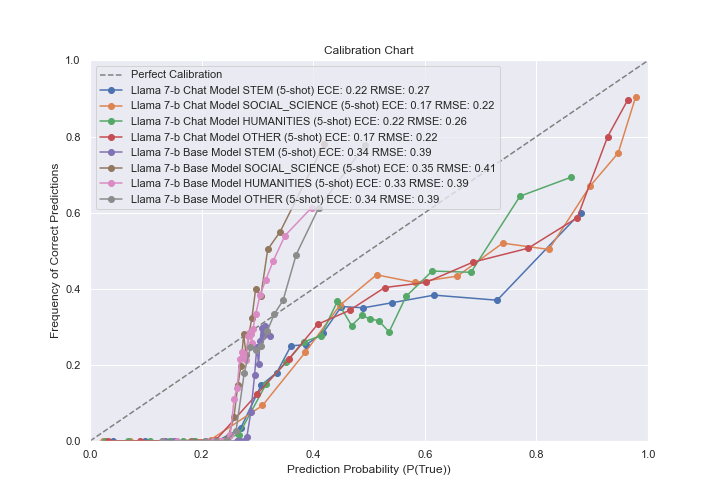
\includegraphics[width=1.1\textwidth]{figures/5-shot-MMLU-subjects-7b.png}
         \caption{\textbf{5-shot MMLU by Subject(7b):}  For subjects which the model can correctly 
         answer few-shot prompting improves accuracy and calibration}
         \label{fig:5-shot-MMLU-subjects-7b}
     \end{subfigure}     
    \hfill 
     \begin{subfigure}[b]{0.38\textwidth}
         \centering 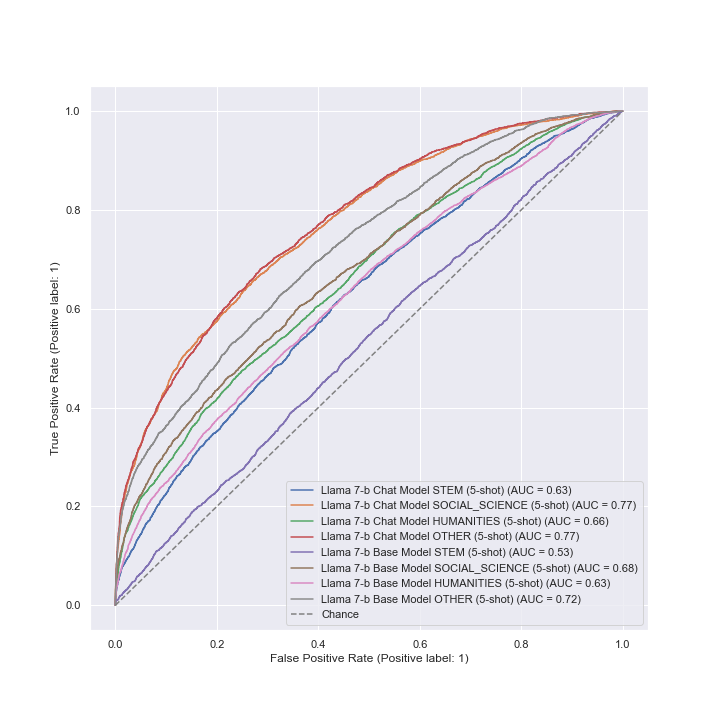
\includegraphics[width=0.9\textwidth]{figures/5-shot-MMLU-subjects-7b-roc.png}
         \caption{\textbf{5-shot MMLU by Subject ROC (7b):} We note large increase in accuracy for 
         Humanities and Other, category with few-shot prompting}
         \label{fig:5-shot-MMLU-subjects-7b-roc}
    \end{subfigure} 
        \caption{Calibration Performance of Chat and Base models on the MMLU multiple choice question answering dataset.}
        \label{fig:MMLU-subjects-7b}
\end{figure*}

\begin{figure*}
     \centering
     \begin{subfigure}[b]{0.60\textwidth}
         \centering 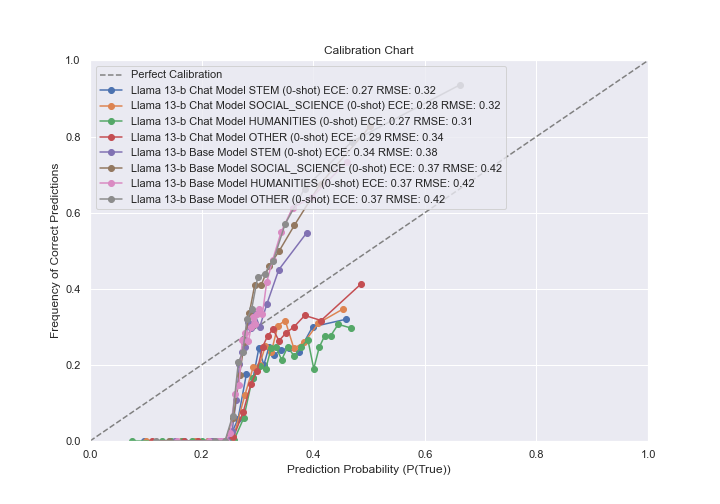
\includegraphics[width=1.1\textwidth]{figures/0-shot-MMLU-subjects-13b.png}
         \caption{\textbf{0-shot MMLU by Subject(13b):}  Base models out perform fine-tuned models, but they are not calibrated and predict lower probabilities for correct answers}
         \label{fig:0-shot-MMLU-subjects-13b}
     \end{subfigure}
     \hfill
     \begin{subfigure}[b]{0.38\textwidth}
         \centering 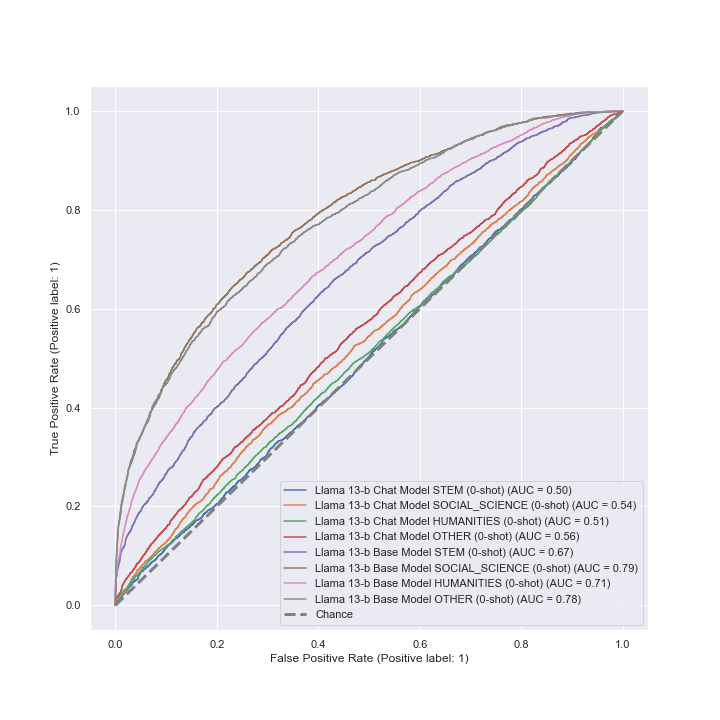
\includegraphics[width=0.9\textwidth]{figures/0-shot-MMLU-subjects-13b-roc.png}
         \caption{\textbf{0-shot MMLU by Subject ROC (13b):} Performance on MMLU shows poor classification, however few-shot prompting enhances classification for subjects the model is predisposed to answer}
         \label{fig:0-shot-MMLU-subjects-13b-roc}
    \end{subfigure}
    
     \hfill
     \begin{subfigure}[b]{0.60\textwidth}
         \centering
         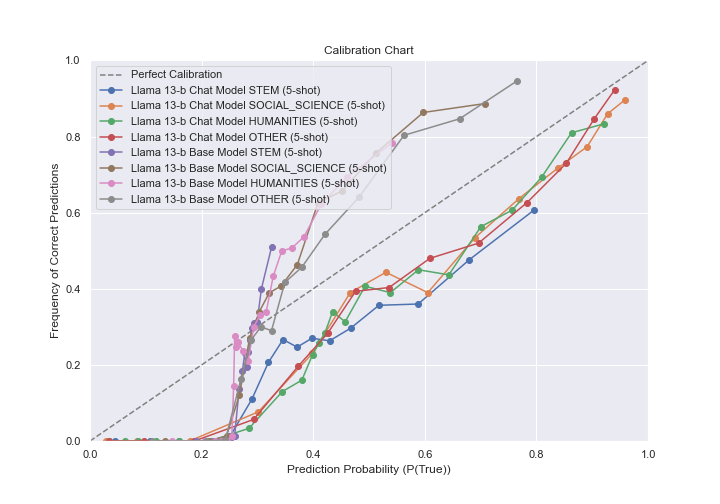
\includegraphics[width=1.1\textwidth]{figures/5-shot-MMLU-subjects-13b.png}
         \caption{\textbf{5-shot MMLU by Subject(13b):}  For subjects which the model can correctly 
         answer few-shot prompting improves accuracy and calibration}
         \label{fig:5-shot-MMLU-subjects-13b}
     \end{subfigure}     
    \hfill 
     \begin{subfigure}[b]{0.38\textwidth}
         \centering 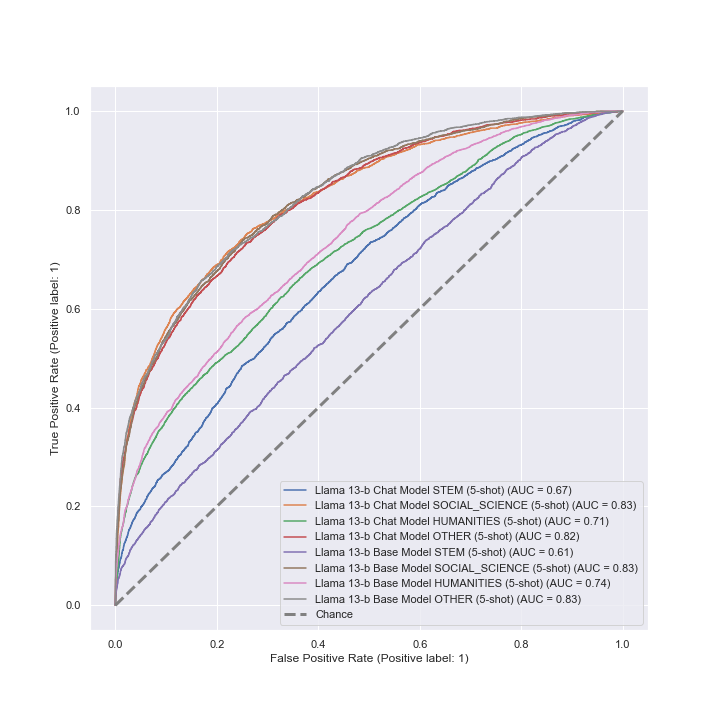
\includegraphics[width=0.9\textwidth]{figures/5-shot-MMLU-subjects-13b-roc.png}
         \caption{\textbf{5-shot MMLU by Subject ROC (13b):} We note large increase in accuracy for 
         Humanities and Other, category with few-shot prompting}
         \label{fig:5-shot-MMLU-subjects-13b-roc}
    \end{subfigure} 
    
        \caption{Calibration Performance of Chat and Base models on the MMLU multiple choice question answering dataset.}
        \label{fig:0-5-shot-MMLU-subjects-13b}
\end{figure*}


\begin{figure*}
     \centering
     \begin{subfigure}[b]{0.60\textwidth}
         \centering 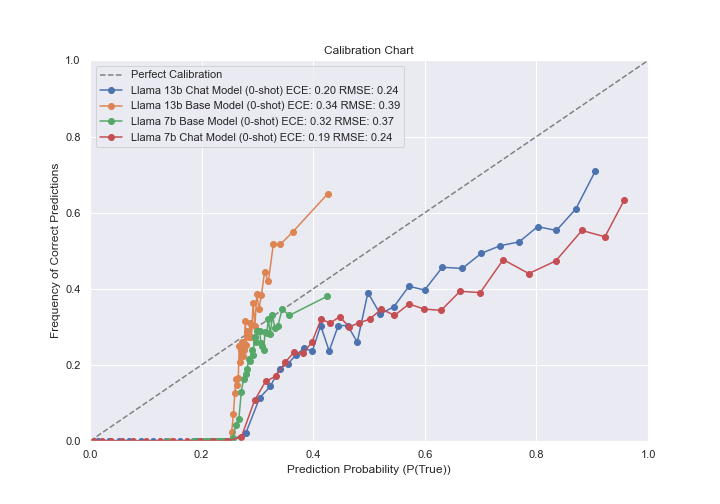
\includegraphics[width=1.0\textwidth]{figures/0-shot-logic-qa.png}
         \caption{\textbf{0-shot Logic QA:} We note the base model under-predicts its performance.} 
         \label{fig:0-shot-logic-qa}
     \end{subfigure}
     \hfill
     \begin{subfigure}[b]{0.38\textwidth}
         \centering 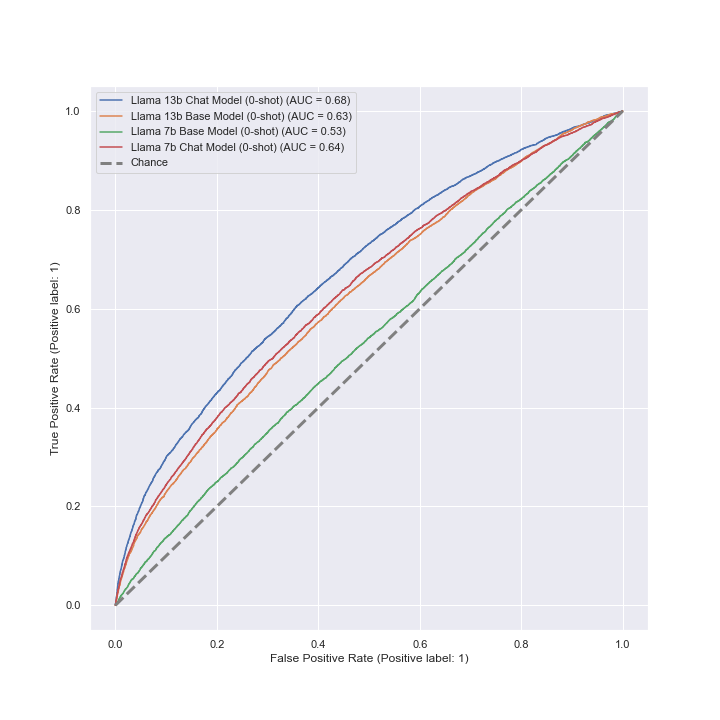
\includegraphics[width=0.9\textwidth]{figures/0-shot-logic-qa-roc.png}
         \caption{\textbf{0-shot Logic QA ROC:} Bigger fine-tuned models show slightly better accuracy}
         \label{fig:0-shot-logic-qa-roc}
    \end{subfigure}  
    
     \hfill
     \begin{subfigure}[b]{0.60\textwidth}
         \centering
         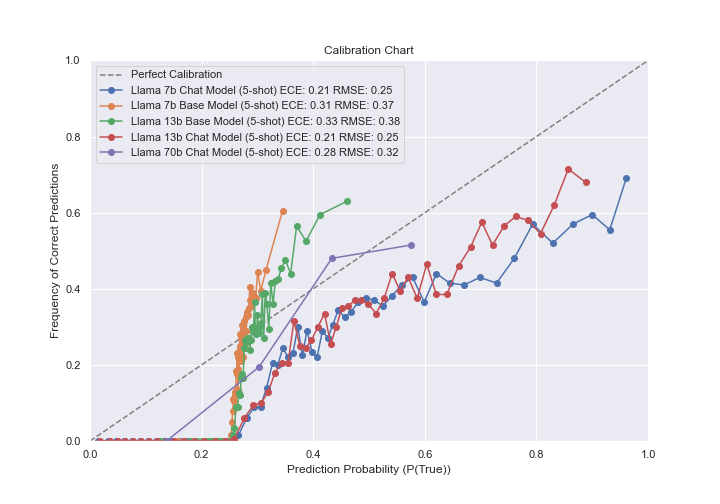
\includegraphics[width=1.0\textwidth]{figures/5-shot-logic-qa.png}
         \caption{\textbf{5-shot Logic QA:} Chat models improve in calibration in 5-shot questioning, much like MMLU. Base models do not show any such improvement.}
         \label{fig:5-shot-logic-qa}
     \end{subfigure}     
    \hfill 
     \begin{subfigure}[b]{0.38\textwidth}
         \centering 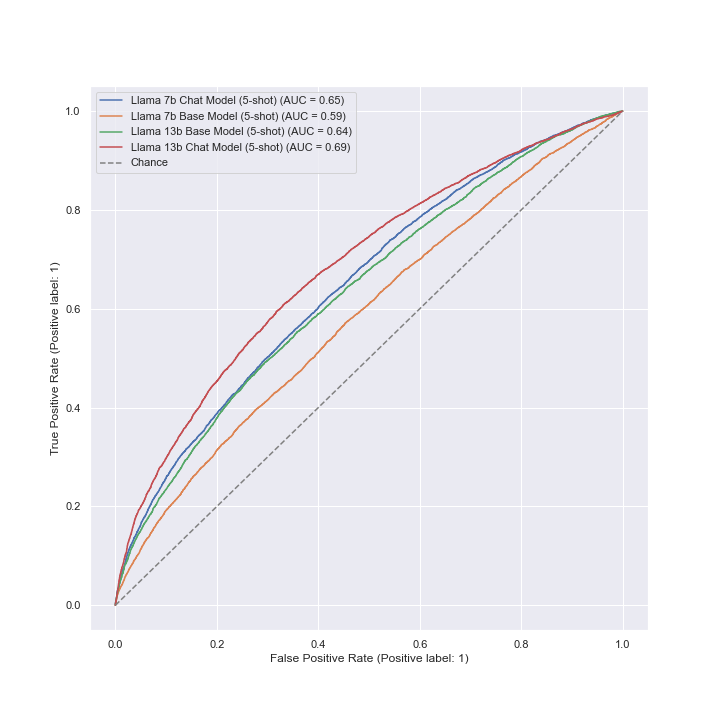
\includegraphics[width=0.9\textwidth]{figures/5-shot-logic-qa-roc.png}
         \caption{\textbf{5-shot Logic QA ROC:}  note that we do not see significant differences in performance before and after prompting. Fine tuning however improves calibration performance},
         \label{fig:5-shot-logic-qa-roc}
    \end{subfigure} 
        \caption{Calibration Performance of Chat and Base models on the LogicQA , logical question answering dataset}
        \label{fig:logic-qa}
\end{figure*}

\begin{figure*}
     \centering
     \begin{subfigure}[b]{0.60\textwidth}
         \centering 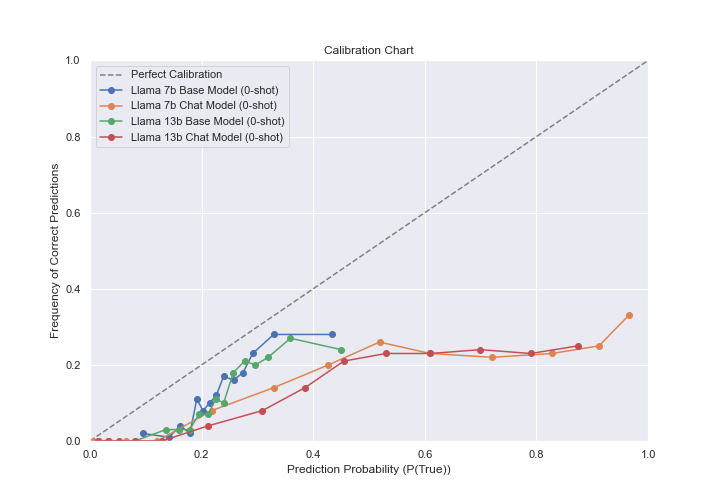
\includegraphics[width=1.0\textwidth]{figures/0-shot-truthful_qa.png}
         \caption{\textbf{0-Shot TruthfulQA:} We note that chat models suffer from overconfidence in 0-shot models, moreover model size fails to show significant improvement on TruthfulQA dataset}
         \label{fig:0-shot-truthful_qa}
     \end{subfigure}
     \hfill
     \begin{subfigure}[b]{0.38\textwidth}
         \centering 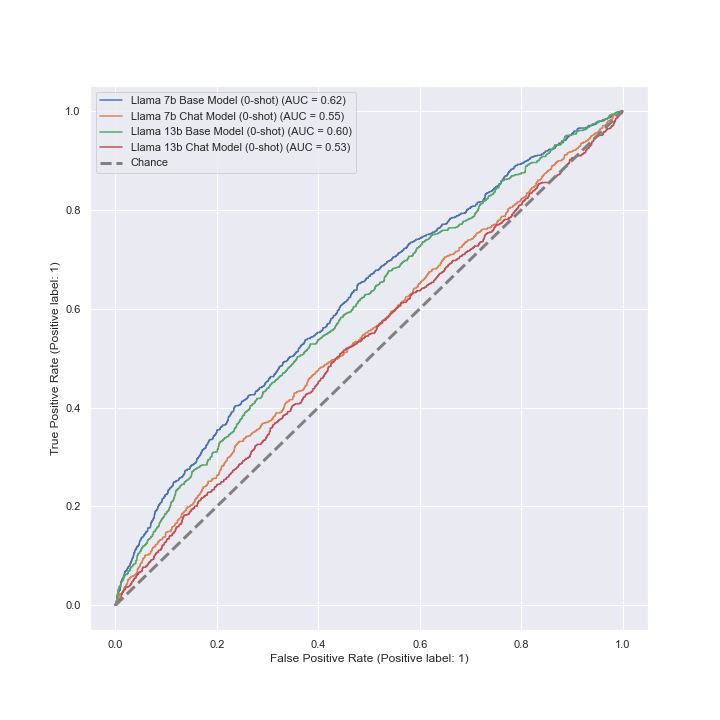
\includegraphics[width=0.9\textwidth]{figures/0-shot-truthful_qa-roc-roc.png}
         \caption{\textbf{0-shot TruthfulQA:} Base models marginally outperform fine-tuned chat models 
         in terms of accuracy},
         \label{fig:0-shot-truthful_qa-roc-roc}
    \end{subfigure} 
     \hfill
     \begin{subfigure}[b]{0.60\textwidth}
         \centering
         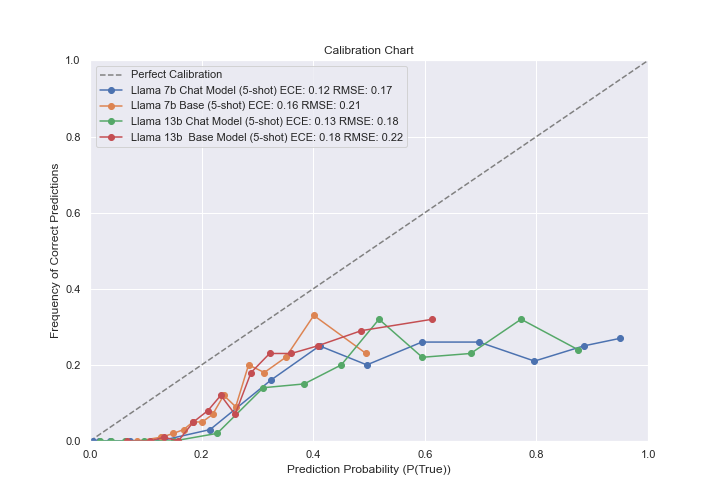
\includegraphics[width=1.0\textwidth]{figures/5-shot-TruthQA.png}
         \caption{\textbf{5-shot Truthful QA:} Truthful QA finds chat models overconfident in their prediction after fine-tuning. No large increase in accuracy or calibration is observed.}
         \label{fig:5-shot-TruthQA}
     \end{subfigure}    
     \hfill
    \begin{subfigure}[b]{0.38\textwidth}
         \centering 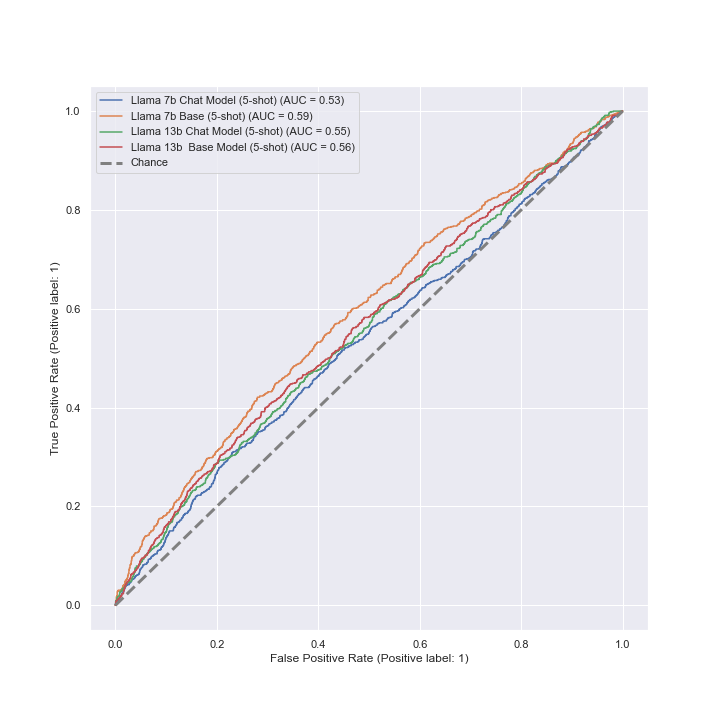
\includegraphics[width=0.9\textwidth]{figures/5-shot-TruthfulQA-roc.png}
         \caption{\textbf{5-shot Truthful QA:}  Multiple shot prompting worsens performance of fine-tuned models},
         \label{fig:5-shot-TruthfulQA-roc}
    \end{subfigure} 
        \caption{Calibration Performance of Chat and Base models on the Truthful QA}
        \label{fig:5-shot-TruthfulQA}
\end{figure*}


%% \section{Acknowledgements}
%% Acknowledgments (optional, should be used to 
%% acknowledge collaboration with other groups or, e.g., 
%% usage of coding & writing assistants, other people’s code etc.)

\section{References}

The software to generate and reproduce the study 
along with the gathered data is publicly available at 
\cite{Nair_Examining_Calibration_Large}. Additional 
report with results on HumanEval \cite{chen2021evaluating}, and GSM8k 
\cite{cobbe2021gsm8k} to be included separately.

%% logicqa  - liu2020logiqa
%% thruthfulqa  - lin2021truthfulqa
%% mmlu - hendryckstest2021 
%% MMLU  - hendrycks2021ethics
%% GSM8K - cobbe2021gsm8k
%% trivia-qa - 2017arXivtriviaqa
%% humaneval - chen2021evaluating

% Entries for the entire Anthology, followed by custom entries
\bibliography{anthology,custom}
\bibliographystyle{acl_natbib}

\appendix
\section{Appendix}



\subsection{Results}



\subsection{Study Materials}

\label{sec:appendix}

\end{document}
